%% This skeleton file requires IEEEtran.cls version 1.6 or later.
%%
\documentclass[conference,letterpaper]{IEEEtran}
% If the IEEEtran.cls has not been installed into the LaTeX system files,
% manually specify the path to it:
% \documentclass[conference]{../sty/IEEEtran}
\IEEEoverridecommandlockouts
\overrideIEEEmargins

% some very useful LaTeX packages include:

\usepackage{cite}      % Written by Donald Arseneau
                        % V1.6 and later of IEEEtran pre-defines the format
                        % of the cite.sty package \cite{} output to follow
                        % that of IEEE. Loading the cite package will
                        % result in citation numbers being automatically
                        % sorted and properly "ranged". i.e.,
                        % [1], [9], [2], [7], [5], [6]
                        % (without using cite.sty)
                        % will become:
                        % [1], [2], [5]--[7], [9] (using cite.sty)
                        % cite.sty's \cite will automatically add leading
                        % space, if needed. Use cite.sty's noadjust option
                        % (cite.sty V3.8 and later) if you want to turn this
                        % off. cite.sty is already installed on most LaTeX
                        % systems. The latest version can be obtained at:
                        % http://www.ctan.org/tex-archive/macros/latex/contrib
%/supported/cite/

\usepackage[dvips]{graphicx}  % Written by David Carlisle and Sebastian Rahtz
                        % Required if you want graphics, photos, etc.
                        % graphicx.sty is already installed on most LaTeX
                        % systems. The latest version and documentation can
                        % be obtained at:
                        % http://www.ctan.org/tex-archive/macros/latex/required/graphics/
                        % Another good source of documentation is "Using
                        % Imported Graphics in LaTeX2e" by Keith Reckdahl
                        % which can be found as esplatex.ps and epslatex.pdf
                        % at: http://www.ctan.org/tex-archive/info/

\usepackage{amsmath}   % From the American Mathematical Society
                        % A popular package that provides many helpful commands
                        % for dealing with mathematics. Note that the AMSmath
                        % package sets \interdisplaylinepenalty to 10000 thus
                        % preventing page breaks from occurring within multiline
                        % equations. Use:
\usepackage{amssymb}

\usepackage{multirow}
\usepackage[left=0.71in,top=0.94in,right=0.71in,bottom=1.18in]{geometry}
\setlength{\columnsep}{0.24in}
% correct bad hyphenation here
%\hyphenation{op-tical net-works semi-conduc-tor IEEEtran}

%New theorems
\newtheorem{fact}{Proposition}
\newtheorem{definition}{Definition}
%New commands
\newcommand{\q}{\mathbf q}
\newcommand{\dq}{\dot {\mathbf q}}
\newcommand{\deltauhand}{\Delta \mathbf {u}_{hand}}
\newcommand{\deltaqarm}{\Delta \mathbf {q}_{arm}}
\newcommand{\qarm}{\mathbf q_{arm}}
\newcommand{\jacobian}{\mathbf J}
\newcommand{\uhand}{\mathbf{u}_{hand}}
\newcommand{\utarget}{\mathbf{u}_{target}}
\newcommand{\xhand}{\mathbf{x}_{hand}}
\newcommand{\qhead}{\mathbf{q}_{head}}
\newcommand{\xtarget}{\mathbf{x}_{target}}

\begin{document}
% paper title
\title{\huge Yet Another Paper}

% author names and affiliations
\author{\authorblockN{Lorenzo Natale}
\authorblockA{
\textit{Italian Institute of Technology}\\
\textit{Via Morego 30, Genova, ITALY}\\
\textit{lorenzo.natale@iit.it}\\}%
\and
\authorblockN{Francesco Nori}
\authorblockA{
\textit{Italian Institute of Technology}\\
\textit{Via Morego 30, Genova, ITALY}\\
\textit{francesco.nori@iit.it}\\}
\and
\authorblockN{Giorgio Metta}
\authorblockA{
\textit{Italian Institute of Technology}\\
\textit{Via Morego 30, Genova, ITALY}\\
\textit{giorgio.metta@iit.it}\\}}%

% make the title area
\maketitle
\begin{abstract}
In this paper we discuss the implementation of a precise reaching controller 
on a humanoid robot upper torso. The proposed solution is completely based 
on a learning strategy which does not rely on \emph{a priori} models of the arm 
and head kinematics. The only major simplification is represented by the 
assumption that a visual model of the hand is available (i.e. the robot 
can visually localize the hand). In fact, from a practical point of view, 
the problem of creating a visual model of the hand is a stand alone problem 
which falls outside the scope of this work.
\end{abstract}

% key words
\begin{keywords}
Development of perceptual and motor systems, machine learning, visual servoing, redundant systems.
\end{keywords}
%
\section{Introduction}
Growing evidence in developmental psychology shows the importance 
of motor activity for cognitive development in humans \cite{gallese06mirror}. 
In particular it is through manipulation that infants gain direct access to objects 
and discover properties that otherwise would remain hidden. 
This concerns for example properties like weight, shape, texture and 
softness that are, if not impossible, at least extremely hard to perceive 
by using visual information alone. In adults information originating 
from motor activity and direct contact with the environment, supports 
perception \cite{klatzky87hand}; during development
the physical interaction with the environment provides infants 
with natural invariances that are useful occasions for learning.
Interestingly, motor and perceptual development seem to follow synchronous  
schedules as if new achievements in the motor system were promoting
the development of new perceptual skills \cite{bushnell93motor}.

Research in developmental robotics has demonstrated the importance of
motor activity (in particular manipulation) for visual and haptic 
perception \cite{fitzpatrick07shared}. One of the 
limitations of these approaches is that controlling the interaction between
the robot and the environment is difficult especially when precise models are
not available. Experiments with robots have thus focused on situations
in which the interaction with objects is relatively simple. For these reasons
the investigation of perceptual development in robots requires addressing 
the problem of motor development first and improving how robots interact
with the world.

In this context we focus on reaching, which is clear prerequisite for 
grasping. If vision of the hand and target were available then this problem 
would be easily solved by employing a visual servoing approach (see 
\cite{hutchinson96tutorial} for a review) which is typically based on 
the use of the visuo-motor Jacobian of the arm. The eye-to-hand Jacobian 
transformation is a function of the arm and head joints and includes knowledge 
of the camera parameters; its estimation is in practice a difficult task.
The fundamental advantage of this approach is that even an inaccurate estimation 
of the Jacobian allows reducing the error of the task to zero. But the visual 
servoing approach is not necessarily the best solution. On one hand delays in 
the control loop pose limitations on the speed of the arm, while on the other 
hand it requires that the hand and target are continuously visible for the 
duration of the movement. 
Reaching can also be performed open-loop by directly relating the joint angles of 
the head with those of the arm \cite{blackburn94learning,metta99developmental}. 
The drawback of this approach is that errors because of modeling inaccuracies and 
noise in the sensors, calculations, actuation, cannot be made arbitrarily small 
as in the visual servoing case.

Results in developmental psychology suggest that both solutions might be
adopted by the brain. Clifton et al. \cite{clifton93isvisually} 
tested whether infants require vision of their hand when reaching; they 
found that infants' ability to touch (and grasp) objects is independent 
of whether sight of the hand is available or not. On the other hand 
other experiments \cite{ashmead93visual} show that later on in development 
there is an increase of visual guidance in reaching. Together these results 
suggest the hypothesis that there are two ``distinct'' reaching mechanism: 
one that relies on ``proprioceptive'' information alone and one that uses 
``visual feedback'' to compensate for errors in the visual domain. Further,
there are studies that show the link of the control of the gaze in relation
to the precision of reaching \cite{flanders-daghestani-berthoz-1999}. 
In this paper we integrate the two modes of control with an approach based on
the hypothesis that the target object is fixated. We use the open loop
controller to bring the hand close to the target. The closed loop controller 
is activated when visual feedback from the hand is available. In practice,
we show that the error could be made arbitrarily small. The problem of 
redundancy in solved in the first case by imposing additional constraints to 
the task. Finally, we describe the procedure by which the robot learns all 
the transformations required by the controllers (the open-loop mapping and 
the arm visual Jacobian).
\section{Previous Works}

%[-] locating an observed object with respect to the robot requires the following data:
%		[*] robot forward kinematic (analytical or estimated)
%	[*] cameras calibration (self or grid calibration)
%[*] hand-eye calibration 

%[-] visual servoing requires:
%	[*] the manipulator jacobian dx_hand = J(q_arm) dq_arm
%[*] the interaction matrix ds = L(q_head, q_arm) dx_hand

In this section we briefly describe previous approaches to the problem of 
performing precise reaching with a robot arm. As stated above, the problem 
naturally splits down into two phases, open loop and closed loop, both well 
studied in literature.

The {\em open loop} phase requires a sensory-motor map encoding the relationship between hand visual localization and arm position. Following a classical procedure, this map can be practically decomposed into three parts: the robot forward kinematics (mapping the hand reference frame into a robot reference frame), the camera projective map (mapping the hand reference frame into a camera reference frame) and the hand/eye map (mapping the camera reference frame into the hand reference frame). Extensive literature has been produced to describe different calibration procedures for retrieving each of these basic maps. Suitable kinematic \cite{Hollerbach96calibration} and hand/eye \cite{Tsai88calibration} calibration procedures can be used to retrieve the forward kinematic and the hand/eye maps. Similarly, different algorithms and strategies have been proposed for cameras and stereo rigs calibration, which is a well known problem `per se', studied mainly in computer vision \cite{Soatto03vision} but with extensive application in robotics. 

Though the final result of these procedures can be extremely accurate, the standard calibration techniques require the robot to operate in an highly structured environment (typically represented by a calibrated grid or object) with a precisely calibrated hand pose sensor (typically a stereo rig), which is not desirable in certain applications. Therefore, alternative procedures have been proposed in order to relax some of the above assumptions. In \cite{AHE01} for example, an hand/eye calibration procedure which does not use any calibration object is proposed. Other approaches have introduced the possibility of performing a kinematic calibration without measuring the hand pose \cite{Bennett91calibration}, but only relying on proprioception and exploiting specific kinematic constraints (e.g. by keeping the hand fixed on the ground).

For certain applications the classical calibration procedures are not 
necessary. A simpler approach \cite{blackburn94learning} avoids the estimation 
of the three maps mentioned above by learning a single forward map. 
In this case
the map links the head joint position to the corresponding arm position that
keeps the hand in fixation. When the robot fixates the target reaching can be 
performed by inverting this map to retrieve the arm command which brings
the hand to the fixation point. Recently this approach has been successfully 
extended to redundant manipulators \cite{lopes06learning}, although in the 
case of a 2-dimensional visual space.

The {\em closed loop} phase requires knowledge of the Jacobian of the open loop map.
It can be derived analytically from 
mathematical differentiation of the function describing the forward map itself. 
Alternatively, some works have proposed techniques to directly estimate the Jacobian matrix
\cite{Hosoda94versatile,Mansard06jacobian} or its inverse 
\cite{Lapreste04efficient}.

In this paper we integrated together the 
open \cite{blackburn94learning,Mansard06jacobian} and closed 
\cite{Hosoda94versatile,lopes06learning} loop 
strategies, both performed in the 3-dimensional space.
We also propose a procedure to estimate 
the Jacobian of the manipulator in the case of a redundant head. All the 
transformations required to perform the task, are autonomously estimated by the robot 
 without relying on any \emph{a  without relying on any \emph{a priori} knowledge about the robot 
kinematic structure.

\subsection{Robotic setup}
In the experiments repored in this paper we used the robot James 
\ref{figJames}. James is a \textit{upper-torso humanoid robot} with the 
size of about ten years old baby. It has 22 Degrees of Freedom (DOFs) 
actuated by 23 motors. Motors are connected to the joints by belts and 
stainless-steel tendonds. The head is equipped with two eyes, which 
can pan and tilt independently (4 DOFs), and is mounted on a 3-DOF 
neck. The arm has 7 DOFs: three of them are located in the shoulder, 
one in the elbow and three in the wrist. The hand has five fingers 
and is under-actuated with a total of 20 degrees of freedom controlled 
by 8 motors. More details on the platform can be found in \cite{JHRAUW06-12}.

\begin{figure}
\centering
\includegraphics[width=2in]{imgs/james.ps}
\caption{James}
\label{figJames}
\end{figure}

\section{Gaze control}
\label{Sec:gazecontrol}

In this section we describe how we control the gaze of the robot to
fixate a visual target.
%
\begin{figure}[tbp]
\centering
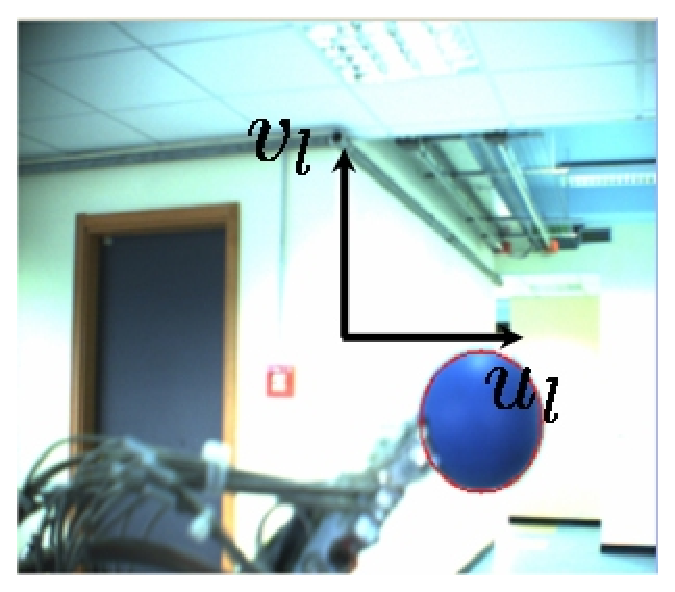
\includegraphics[width=25mm]{Figure/LeftImage.eps} \hspace{1cm}
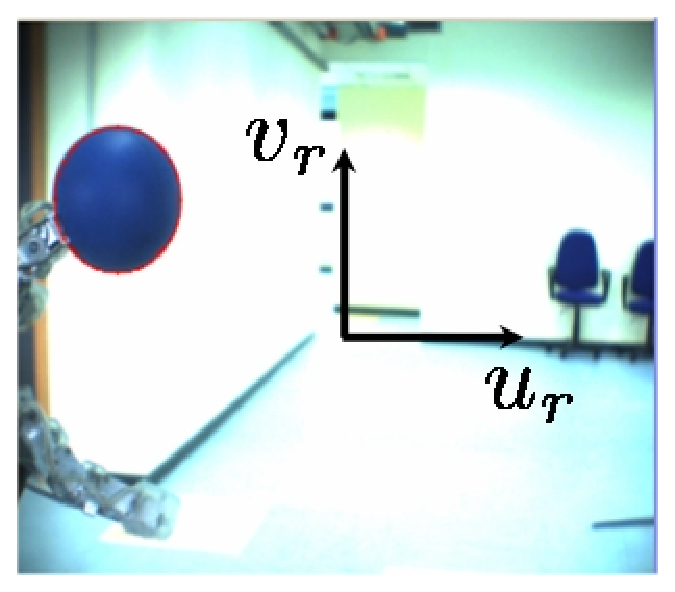
\includegraphics[width=25mm]{Figure/RightImage.eps}
\caption{Two typical images taken from the two cameras mounted on the 
eyes of the robot (resolution 320$\times$240). 
The coordinates of the target (the blue ball) on the image planes
will be denoted $u_r$, $v_r$, and $u_l$, $v_l$ (respectively right 
and left cameras).}
\label{Fig:ImagePlane}
\end{figure}
% 
The crucial aspect in this case concerns the redundancy of the 
head. Let $u_r$ and $v_r$ be the coordinates of the target on the 
right image plane. Similarly, let $u_l$ and $v_l$ be the coordinates 
of the target on the 
left image plane (see Figure \ref{Fig:ImagePlane}). The values of $u_r$, 
$v_r$, $u_l$, $v_l$ are the output of a visual module which detects the
target in the image planes. Directing gaze 
toward the target 
consists in moving the neck and the eyes so as to obtain 
$u_r=0$, $v_r=0$, $u_l=0$, $v_l=0$. 
Let us define the vector 
$\tilde {\mathbf u}_{target}= \begin{bmatrix} u_r & v_r & u_l & v_l 
\end{bmatrix}^\top \in \mathbb R^4$ corresponding to the 
target location in the image planes. Under reasonable 
assumptions, we do not need to impose simultaneously 
the four conditions $u_r=0$, $v_r=0$, $u_l=0$, $v_l=0$.  Our control task 
can be redefined as the problem of controlling 
$\utarget = \begin{bmatrix} u_r & u_l & v_l \end{bmatrix}^\top \in \mathbb R^3$ 
to zero. Clearly, the task specification does not constrain all the head degrees of 
freedom (we are imposing $m=3$ constraints but we have $n=6$ free variables 
available: we remain with $n-m=3$ additional degrees of freedom). 
The strategy we have chosen to solve this ``redundancy problem'' consists in 
using two controller for the eyes and the neck. The former controls 
the eyes version and common tilt to track the object, while the latter
controls neck yaw and pitch to maintain the eyes ``centered'' within 
the neck. Mathematically the above strategy can be implemented 
as follows:

\begin{eqnarray} \label{Eq:HeadEyeControl}
\left\{\begin{matrix}
\dot {\alpha_v^c} &=&   K_p (u_l + u_r)\\
\dot {\theta_y} &=&   K_y \alpha_v^c 
\end{matrix}
\right.,\quad
\left\{ \begin{matrix}
\dot {\alpha_t^c} &=&   K_t (v_l + v_r)\\
\dot {\theta_p} &=&   K_r \alpha_t^c
\end{matrix} \right.,
\end{eqnarray}
%
where $\alpha_t^c$ and $\alpha_v^c$ are the eyes version and common tilt and 
where $\theta_y$ and $\theta_p$ are the yaw and pitch movement of the neck. 
In the proposed control scheme, the vergence degree of freedom $\alpha_v^d$, 
which corresponds to the distance of the target does not influence 
the neck position and is therefore controlled separately from the neck:
\begin{eqnarray} 
\dot {\alpha_v^d} &=&   K_p (u_l - u_r).
\end{eqnarray}
Finally, the neck roll degree of freedom $\theta_r$ is maintained fixed, 
i.e. $\theta_r^d=0$.

The proposed control strategy allows us to asymptotically fixate the target 
($u_l \rightarrow 0$, $v_l \rightarrow 0$, $u_r \rightarrow 0$ which 
implies $v_r \rightarrow 0$) while also guaranteeing an asymptotically 
straight gaze ($\alpha_v^c \rightarrow 0$, $\alpha_t^c \rightarrow 0$). Moreover, 
by choosing a suitable value for the gains $K_p$, $K_y$, $K_t$ and $K_r$ it
is possible to achieve an asymptotic behavior with the eyes moving rapidly on 
the target and the neck following the eye movement with a slower 
movement.

\section{Reaching}
\label{sec:reaching}

In this section, we describe the two approaches we followed to solve
the reaching task on our robot. The first method 
uses the forward mapping between the arm joint space and the three 
dimensional position of the hand represented in the head reference 
frame. The second method uses a visual servoing technique to control the 
speed of the arm to minimize the position of the hand in the 
image plane with respect to a desired target (the fixated object).

\subsection{Open Loop Reaching} \label{sec:openReaching}
%
Suppose that the robot is tracking a target as described 
in Section \ref{Sec:gazecontrol}. In the assumption of perfect 
tracking (the visual error is zero), the three dimensional spatial position 
of the target with respect to the robot, denoted $\tilde {\mathbf x}_{target} 
\in \mathbb R^3$, 
is a function of the head configuration $\mathbf q_{head} =
\begin{bmatrix} \theta_y & \theta_p & \theta_r & \alpha_v^d & \alpha_v^c & \alpha_t^c \end{bmatrix}^\top \in \mathbb R^6$.
However, the representation of the target position, 
$\tilde {\mathbf x}_{target}$, in terms of the full head configuration, 
$\mathbf q_{head}$, is clearly redundant.
Specifically, the same target position can be represented by different 
head configurations. To obtain a one to one mapping between the target 
position and the head configuration we have to analyze the 
gaze controller. The latter maintains $\theta_r$ stationary 
($\theta_r^d = 0$) and poses additional constraints on the head joints. 
In particular we know from section \ref{Sec:gazecontrol} that the 
controller minimizes $\alpha_t^c$ and $\alpha^c_v$ (see equation 
(\ref{Eq:HeadEyeControl})) so that they asymptotically
converge to zero ($\alpha_t^c \rightarrow 0$ and 
$\alpha_v^c \rightarrow 0$). Ideally, after 
fixation is achieved, we have $
\mathbf {q}_{head}=
\begin{bmatrix} \theta_y & \theta_p & 0 & \alpha_v^d & 0 & 0 \end{bmatrix}^\top \in \mathbb R^6.
$
%
Since there exists a one to one mapping between the three dimensional 
position of the target 
$\tilde {\mathbf x}_{target}$ and the three non-zero variables 
$\theta_y$, $\theta_p$ and $\alpha_v^d$, we can define $
\mathbf x_{target}=
\begin{bmatrix} \theta_y & \theta_p & \alpha_v^d\end{bmatrix}^\top \in \mathbb R^3.
$
%
This new variable $\mathbf x_{target} \in \mathbb R^3$ uniquely codes the 
spatial position of the target in a way that resembles a three dimensional 
polar representation. In particular $\theta_y$ and $\theta_p$ code 
respectively \emph{azimuth} and \emph{elevation}, while \emph{distance} is 
substituted with $\alpha_v$ (the \emph{vergence} angle). 

If the robot tracks the hand, the same subset of the head joint space 
can be used to code the spatial location of the hand: $
\xhand=
\begin{bmatrix} \theta_y & \theta_p & \alpha_v^d\end{bmatrix}^\top \in \mathbb R^3.
$
%
Under these assumptions, the \emph{forward mapping} 
$f_{arm} : \mathbb R^4 \longrightarrow \mathbb R^3$
relates the arm configuration $\qarm$ with the position of the hand 
$\xhand$:
%
\begin{equation} 
\label{Eq:forward}
\mathbf x_{hand}=f_{arm}(\mathbf q_{arm}), \qquad f_{arm} : \mathbb R^4 \longrightarrow \mathbb R^3.\end{equation}
%
In the next section we show how a neural network could be trained to approximate
the arm forward mapping (Eq. \ref{Eq:forward}).

Suppose now that the robot is fixating a target and that we want to control 
the robot to reach for it. Formally the problem can be formulated 
as determining the value of $\qarm$ which solves the 
following optimization problem:
%
\begin{equation} 
\label{Eq:reaching1}
  \displaystyle\min_{\qarm} \left(J\right)=\displaystyle\min_{\qarm}
  \left\|\mathbf x_{hand} - \mathbf x_{target}\right\|^2,
\end{equation}
%
where $\mathbf x_{target}$ is measured from the encoders of the head, while 
$\mathbf x_{hand}$ is computed from $\qarm$ through Eq. (\ref{Eq:forward}).
Given the redundancy of the arm kinematics the minimization 
(\ref{Eq:reaching1}) has infinite solutions. We constrained the problem by 
forcing one of the joints, for example joint number 2 (one of the shoulder joints), to remain as close 
as possible to a predefined value $q_{20}$:
%
\begin{equation} 
\label{Eq:reaching2}
  \displaystyle\min_{\qarm}\left(J_c\right)=\displaystyle\min_{\qarm}
  \left[
  \left\|\mathbf x_{hand} - \mathbf x_{target}\right\|^2 + \left(q_{arm,2}-q_{20}\right)^2
  \right].
\end{equation}

The optimization of (\ref{Eq:reaching2}) can be performed numerically using 
various algorithms. In our implementation, we used 
the downhill simplex method \cite{ne:Computer:65} as implemented in 
\cite{mo:Press:90}.

\subsection{Learning the open loop reaching} 
\label{sec:learning-open-loop}
%
To learn the forward map of Eq. (\ref{Eq:forward}) we programmed 
the robot to perform random movements with the arm (chosen to uniformly sample 
a predefined region in the robot workspace). During this ``exploratory'' 
phase the robot tracked the hand, and collected samples of the form: $
%
\left(\begin{array}{cc}
  \qarm^i , \xhand^i\end{array}\right)_{i = 0,1\dots}$.
%
 A neural network was then trained to learn the relation:
%
\begin{equation} 
  \xhand=\hat{f}_{arm}\left(\qarm \right),
\end{equation}
%
which approximates Eq. (\ref{Eq:forward}).

In the experiment reported in this paper we collected a data set of 
about 2890 samples that we divided in a training set ($N_{train}=2168$
 samples) and 
a test set ($N_{test}=725$ samples). The neural network we employed was the 
Receptive Field Weighted Regression model proposed 
by \cite{schaal98Constructive}. This network implements an online learning
method, meaning that a learning step is performed every time a new 
sample is presented to the network. All samples in the training set were shown
to the network in a random order. After each training step the 
performance of the network was validated on the whole test set, by computing
the Mean Squared Error (\emph{MSE}) between each sample in the test set, 
$\xhand^i$, and the corresponding network output, 
$\mathbf{\hat{x}}_{hand}^i$:
%
\begin{equation}
\emph{MSE}=\frac{1}{N_{test}}\sum_{i=0}^{N_{test}-1}\|\xhand^i- \hat{\mathbf{x}}_{hand}^i\|^2
\end{equation}
%
The plot in figure \ref{Fig:learningerrors}
shows the trend of the error on the test set during learning. At the end of
the training the network reached the performance of $\emph{MSE}=5.7$ 
(with $\emph{STD}=10.4$).

In the experiment reported in this paper the network was trained offline. 
This was done to simplify the analysis of the results and to perform cross-validation 
on a predefined test set. However, the learning algorithm we used is purely 
incremental (each sample was shown to the network only once and immediately 
discarded), so in this regard it would be straightforward to convert the 
same approach to an online implementation.

\subsection{Closed Loop Reaching} \label{Eq:ClosedLoop}
%
If the robot could visually measure the distance
between the hand and the target, then reaching could also be solved
visually, by implementing a closed control loop. The underlying idea consists in
performing a preliminary (open loop) reaching movement and then refining the action
by visually correcting any residual error. 

We know that the Jacobian matrix relates arm velocities $\dot {\mathbf q}_{arm}$
with hand velocities in the image plane $\dot {\mathbf u}_{hand} = \left[ 
\begin{array}{ccc}
  \dot u_r & \dot u_l & \dot v_{l}
\end{array} \right]^\top$:
\begin{equation} 
  \dot {\mathbf u}_{hand}=
  \tilde{\mathbf J}\left(\mathbf q_{arm}, \mathbf q_{head}\right)
  \dot {\mathbf q}_{arm},
\end{equation}
where $\tilde{\jacobian} \in \mathbb R^{3 \times 4}$ depends on 
both the configuration of the arm and the head. In practice, assuming 
sufficiently small arm movements $\deltaqarm$, we can use the following 
approximation:
%
\begin{equation} 
\label{eq:jacobian1}
  \deltauhand=
  \tilde{\mathbf J}\left(\mathbf q_{arm}, \mathbf q_{head}\right)
  \deltaqarm,
\end{equation}
where $\deltauhand$ = $[ \Delta u_r$, $\Delta u_l$, $\Delta v_{l}]^\top$
is the image plane displacement resulting from the arm movement $\deltaqarm$. 
Due to the additional constraints posed by the head tracker, we showed
that only a subset of $\qhead$, $\xtarget$, is 
sufficient to uniquely identify the position of the head, so we 
can rewrite equation (\ref{eq:jacobian1}) as:
%
\begin{equation}
\label{eq:jacobian2}
  \deltauhand=
  \tilde{\jacobian}\left(\qarm, \xtarget\right)
  \deltaqarm, \qquad \tilde{\jacobian} \in \mathbb R^{3 \times 4}.
\end{equation}
%

Moreover, after the preliminary open loop reaching movement, we know
that $\xtarget = \hat f(\qarm)$ so that  Eq.
(\ref{eq:jacobian2}) can be further simplified to:
%
\begin{equation} 
\label{eq:jacobian3}
  \deltauhand=
  \jacobian \left(\qarm\right)
  \deltaqarm,\qquad \jacobian \in \mathbb R^{3\times4}
\end{equation}
%
where $\jacobian$ depends only on the arm joint configuration $\qarm$.

Suppose now that the robot has to reach for an object, whose visual position is 
represented by $\utarget$. To solve this problem 
the controller of the arm needs to compute the arm command which minimizes 
the error:
%
\begin{equation}
  e=\left\|\uhand-\utarget\right\|^2.
\end{equation}
%
When the head tracker has achieved convergence on the object, 
$\utarget \approx 0 $ and $e$ $\approx \left\|\uhand\right\|^2$.
Due to the redundancy of the arm, the minimization of $e$ can have
infinite solutions. Among them, the minimum norm solution corresponds
to the minimum joint speeds, that is:
%
\begin{equation}
\mathbf{\dot q}_{arm}=-k \cdot \jacobian^\# \uhand, 
\qquad \jacobian^\# \in \mathbb R^{4 \times 3},
\end{equation}
%
where $\jacobian^\#$ is the Moore-Penrose pseudo-inverse of $\jacobian$.

\subsection{Learning the Arm Jacobian}
%
In the previous section we used the Jacobian of the manipulator
$\jacobian$ (actually its pseudo-inverse $\jacobian^\#$) to 
control the arm to reach for a visually identified object. In 
this section we describe a procedure by which the robot can 
autonomously acquire $\jacobian$ and $\jacobian^\#$.

As described in Section \ref{sec:learning-open-loop}, the robot 
moves the arm randomly, while maintaining gaze on the hand. At 
the end of each movement $j$ the arm is in a configuration 
$\qarm^j$,  while the eyes are fixating the hand 
($\uhand \approx 0$) with a straight gaze
(the head tracker has reached convergence). Each 
arm configuration corresponds to a different value of 
$\jacobian_j=\jacobian\left(\qarm^j\right)$. 
Now the robot inhibits the head tracker and performs a sequence $m$
of small arm movements $\deltaqarm^k$ which perturb $\uhand$ of small amounts $\deltauhand^k$:$
  \left(\begin{array}{cc}
    \deltauhand^k , 
	\deltaqarm^k \end{array}
  \right)_{k = 0,1\dots,m}
$. All $m$ perturbations $\deltauhand^k$ and 
$\deltaqarm^k$ are linearly related through $\jacobian_i$ 
as described in Eq. (\ref{eq:jacobian2}). From these $m$ 
observations we can derive a least squares estimation of $\jacobian_j$ from 
which, in turn, we can compute the pseudo-inverse $\jacobian_j^\#$. 

Re-iterating this procedure leads to the collection of a series of examples:
$  \left(\begin{array}{cc}
    \qarm^j , \jacobian_j^\# \end{array}\right)_{j = 0,1\dots}$.
An approximation $\hat{\jacobian}^\#$ of $\jacobian^\#$ is finally
obtained by training a neural network:
%
\begin{equation}
\mathbf{g}\left(\qarm\right), \qquad g : \mathbb R^4 \longrightarrow \mathbb R^{12},
\end{equation}
%
whose output components are the coefficients of 
$\hat{\jacobian}^\# \in \mathbb R^{4 \times 3}$.

We report here the result of a learning session. The robot explored 210 
different arm positions $\qarm^j$ randomly distributed within a region of 
the workspace. In each of these positions the robot executed $m=10$ 
perturbations $\deltaqarm^k$ and estimated an example $\jacobian^\#_j$ for 
the neural network. Overall we collected 210 samples for $\jacobian^\#$. 
We trained the neural network on a subset of $N_{train}=158$ elements 
(training set); each 
sample was shown to the network only once and then discarded. Following each 
training step, we evaluated the performance of the network by computing 
\emph{MSE} on the remaining $N_{test}=52$ elements 
(test set). At the 
end of the training the error on the test set was $\emph{MSE}=2$ 
($\emph{STD}=7.1$). Figure \ref{Fig:learningerrors} reports the plot of 
the error during learning.
%
\begin{figure}
  % Requires \usepackage{graphicx}
  \begin{center}
	\begin{tabular}{ccc}
	  \parbox{30mm}{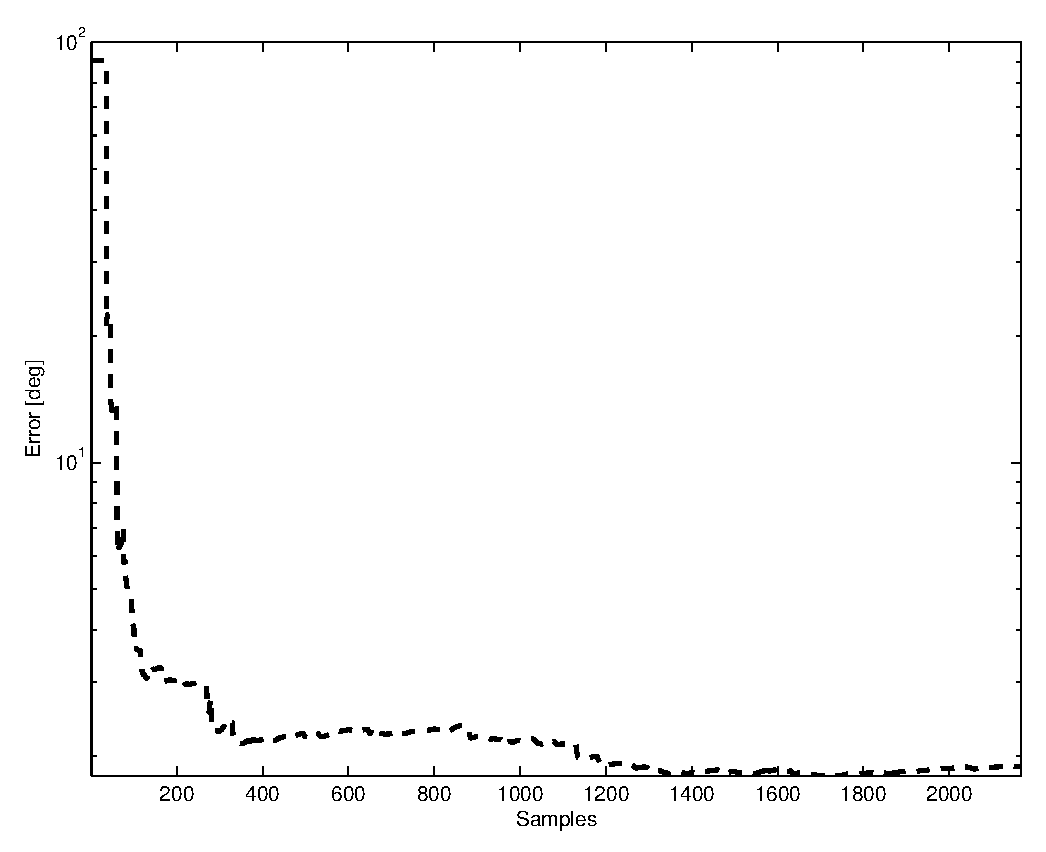
\includegraphics[width=35mm]{./Figure/reachingError1.eps}}  & \hspace{.1cm} &
	  \parbox{30mm}{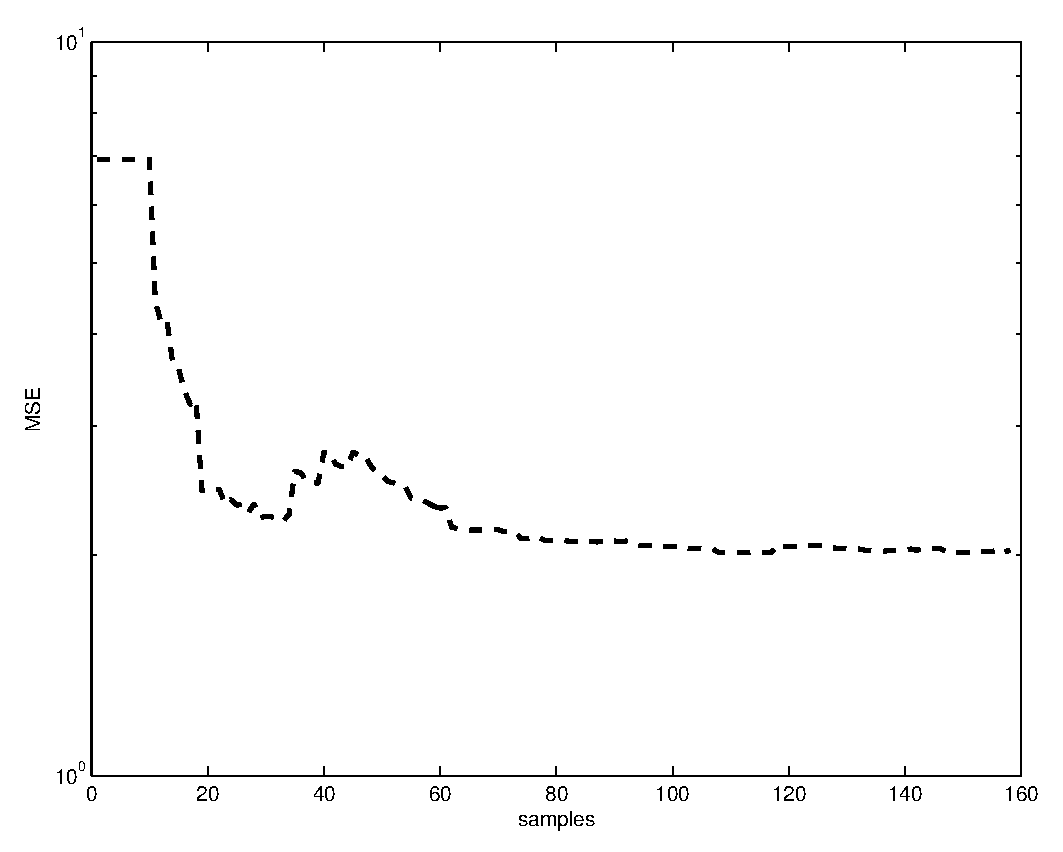
\includegraphics[width=35mm]{./Figure/jacobian-error.eps}}
  \end{tabular}
\end{center}
\caption{Left: learning of the arm forward function. Right: learning the 
arm jacobian. The plots represent the \emph{MSE} on 
the test set during learning. See text for more details}\label{Fig:learningerrors}
\end{figure}


\section{Results}
\label{sec:results}

\begin{table*}[tb]
  \caption{Objects} \label{tab:objects} \centering
  \begin{tabular}{|c|l|c|c|c|l|}
    \hline
    &Description& Weight(Kg)&No.Trials&No.Failures&Contains \\
    %&Object& W(Kg)&Trials&Fail&Contains \\
    \hline
    1&White Bottle        & 0.265 & 22& 0 & Vitamins\\
    2&White Porcelain cup & 0.255 & 24& 1 & Nothing\\
    3&Startbucks cup      & 0.220 & 24& 4 & Bolts \\
    4&Nesquick box        & 0.240 & 24& 2 & Nesquick powder\\

    \hline
  \end{tabular}
\end{table*}

\begin{figure}[tbp]
\centerline{
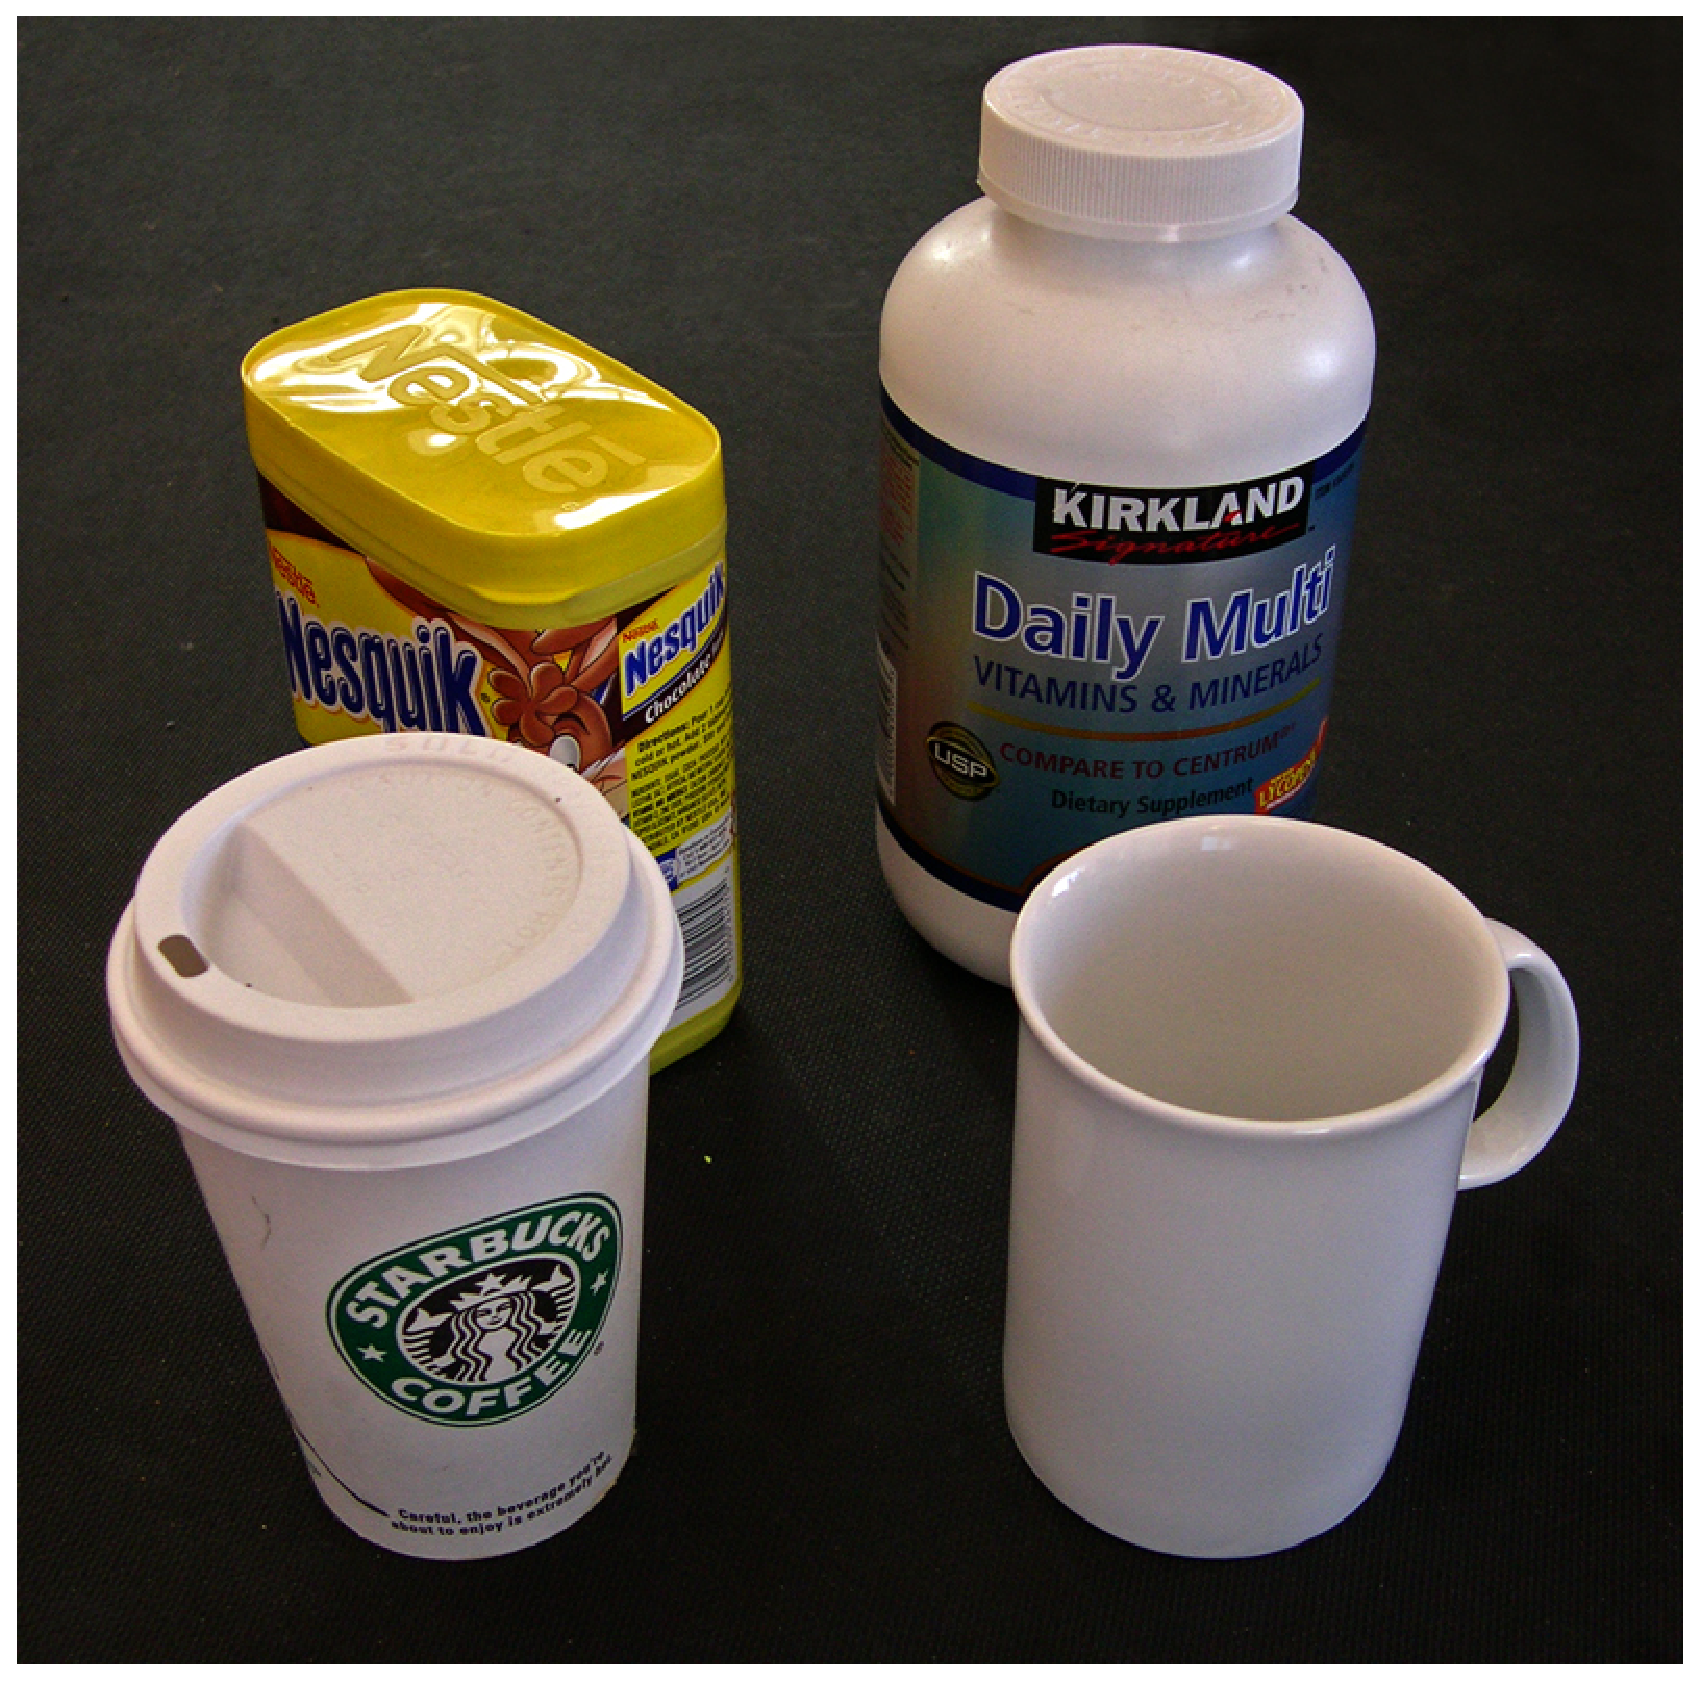
\includegraphics[width=2.0in]{./figures/objects.eps}
}\caption{Objects}
\label{fig:Objects}
\end{figure}

An example resulting from the implementation described in
section~\ref{sec:behavior} is shown in figure~\ref{fig:sequence}.
We can observe the reaching action followed by the positioning and
grasping. [Should we include a plot of the readings of the
sensors?]


Using the behavior described in section~\ref{}, the robot was able
to grab a number of different objects. The robot had no prior
knowledge of the objects. We evaluate the performance by
presenting to the robot many times four objects and counting the
number of times that they were grabbed. Out of 94 trials only 8
failed. The objects were : a white vitamins bottle, a white
porcelain cup, a startbucks cup and a nesquick box. The physical
properties of the objects and the results are shown in table
\ref{tab:objects}.

[No sure if we should include this part]

We have also evaluated the behavior of the tactile sensor grabbing
the same object but with different weights. The object used was
the white bottle and the weights used are presented in the
table~\ref{}.






%We evaluated our work by performing an object recognition
%experiment. We exposed the robot one evening to a set of seven
%objects, and then in the morning tested its ability to recognize
%another set, which had an overlap of four objects with the
%training set. Three of these objects were chosen (Figure 8) to
%represent three different materials, plastic, glass and steel
%(metal). The idea is that the sound produced by each object
%depends on its size, shape and the material with which it is made;
%accordingly we expected the tapping to produce three different
%distinct sounds. A fourth object (a plastic toy) was relatively
%silent. For each run, we placed randomly selected objects on the
%table in front of the robot, and it was responsible for finding
%and tapping them. Overall the robot tapped 53 times; of these
%episodes 39 were successful, meaning that the sound produced by
%the tapping was significantly loud; in the other 14 cases the
%tapping did not provoke useful events either because the initial
%impact caused the object to fall, or the object remained too close
%to the hand. The high number of successful trials shows that given
%the mechanical design of the hand, haptic feedback was sufficient
%to control the interaction between the robot and the environment.
%We evaluated the performance of our spectrum comparison method by
%ranking the strength of matches between episodes on the second day
%and episodes on the first day. Figure 7 shows what detection
%accuracy is possible as the acceptable false positive rate is
%varied. This predicts that we can on average correctly match an
%episode with 50\% of previous episodes involving the same object
%if we are willing to accept 5\% false matches.

\section{Conclusions}
In this paper we have described the implementation of a reaching
behavior that integrates together an open loop and a closed 
loop controller. The open loop controller
allows the robot to perform faster movements and does not require visual 
feedback from the hand. When sight of the hand is available the closed
loop controller allows for precise positioning of the hand in the 
image plane. The procedure among the other things estimates the eye-to-hand
visual Jacobian of the robot. In this respect our method provides
similar results to the ones described in the literature \cite{}

We describe an explorative strategy by which the robot autonomously 
acquires the transformations required to control the hand to reach for a
visually identified target.

We do not rely on any prior information about the 
parameters of the robot. The only simplification was that we used 
a color mark to visual localize the hand of the robot. Our assumption
is that the hand localization/identification is a separate problem
that needs to be solved before learning reaching. Previous work
by the same and other authors have suggested procedures by which 
the robot could autonomously learn to solve this task 
(\cite{Natale05,edsinger06what}). It will be interesting to see
how these approaches can be integrated with the work described 
in this paper.

\section*{Acknowledgement}
% optional entry into table of contents (if used)
%\addcontentsline{toc}{section}{Acknowledgment}
The work presented in this paper
has been supported by the \textsc{RobotCub} project, funded by the
European Commission through Unit E5 ``Cognition''. Moreover, it has
been partially supported by \textsc{Neurobotics}, a European FP6 
project (IST-2003-511492).




%

% references section
%%% this must be IEEEtran
\bibliographystyle{IEEEtran}
\bibliography{main}

\end{document}




